\chapter{3D画像の半教師あり学習による,少量ラベルの腫瘍と正常の分類}

\section{胃がんの画像データ取得方法}

\subsection{透明化と染色}
ホルマリン固定されている検体をLUCIDによる透明化してから染色する.
多光子顕微鏡で3D画像として撮影する.一つの視野で観察することができる領域は縦横が~で深さ方向が~である.ここでLUCIDによる透明化によって今までは断面のみの撮影だったものを深さ方向まで撮影することができるようになった.
検体全ての撮影をするために画像取得にはタイリングをする.

% 三次元に撮影した画像

\begin{figure}
	\centering
	\subfigure[]{
		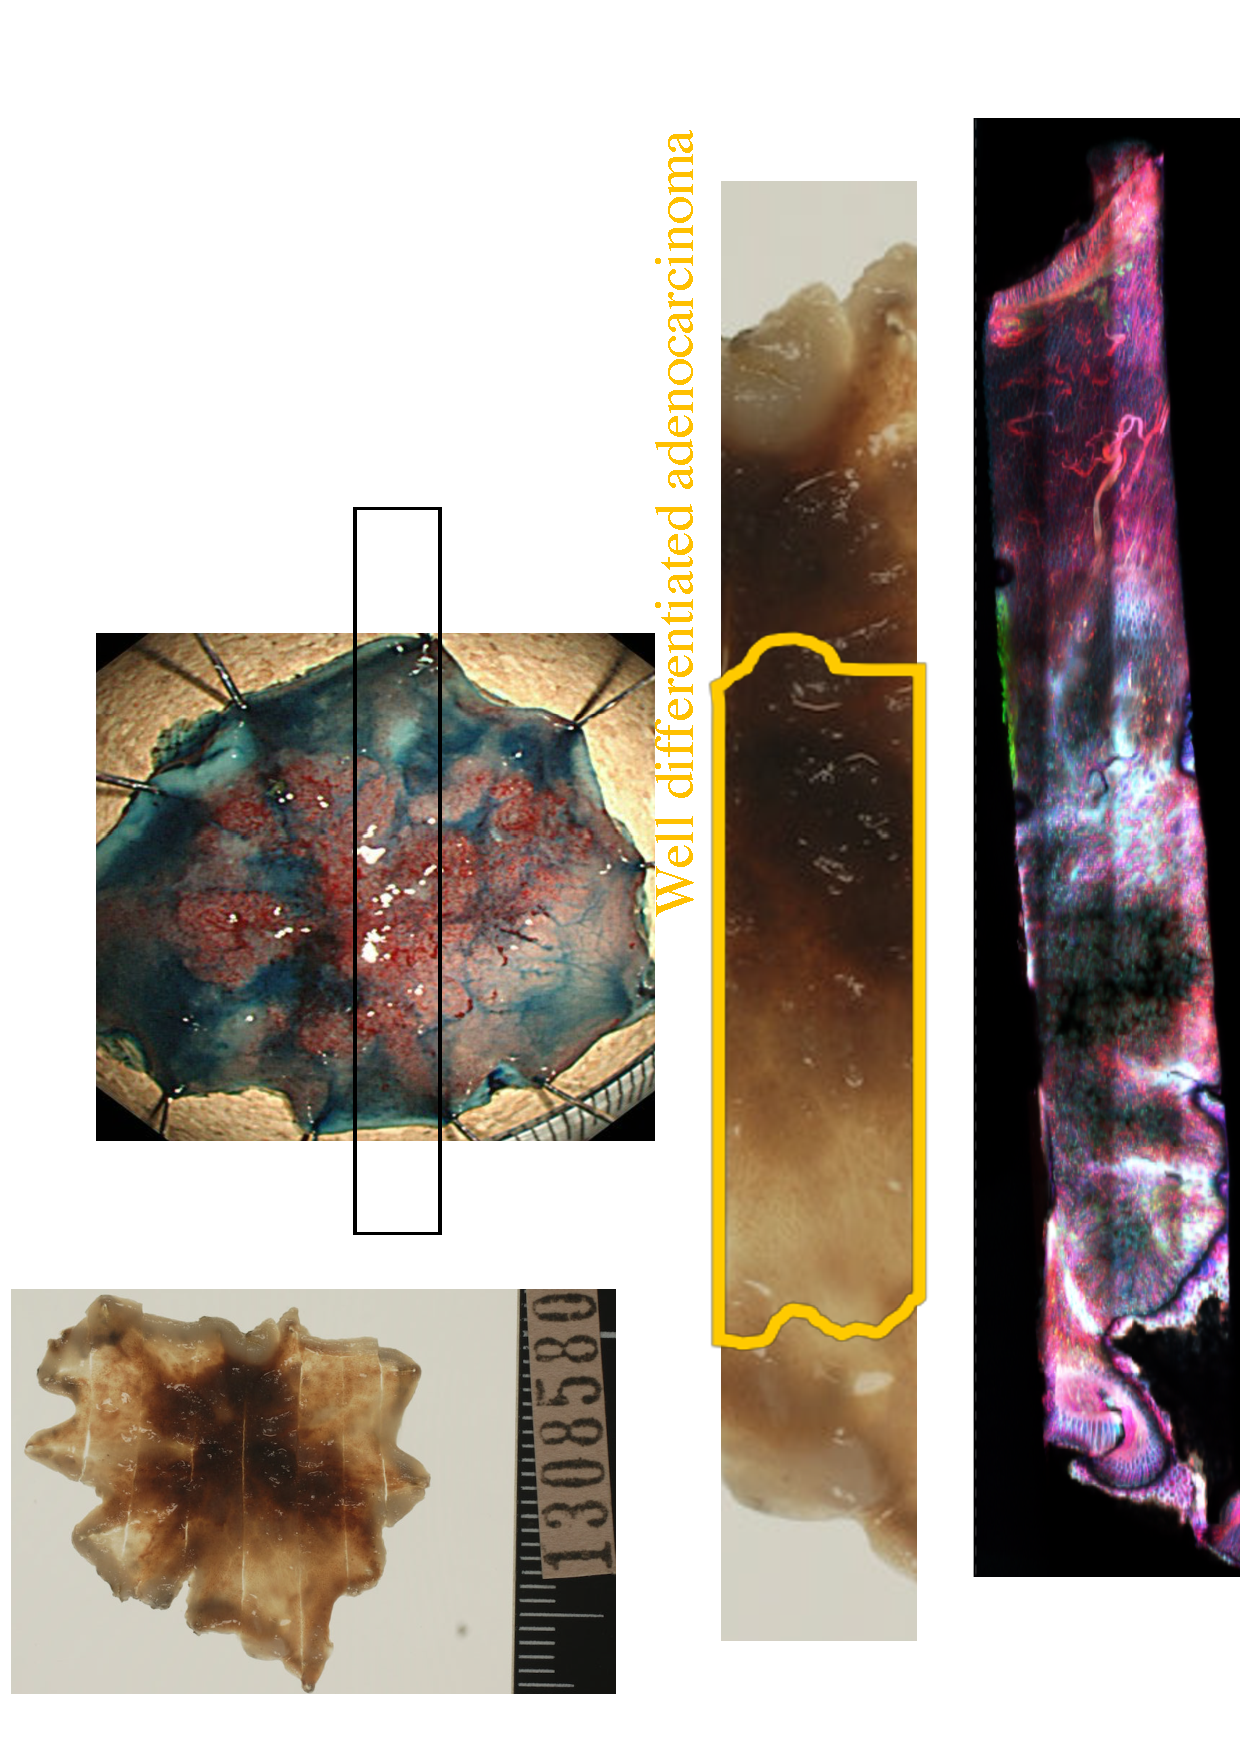
\includegraphics[clip, width=0.4\linewidth]{fig/raw_data/summary/C-009}
	}
	\subfigure[]{
	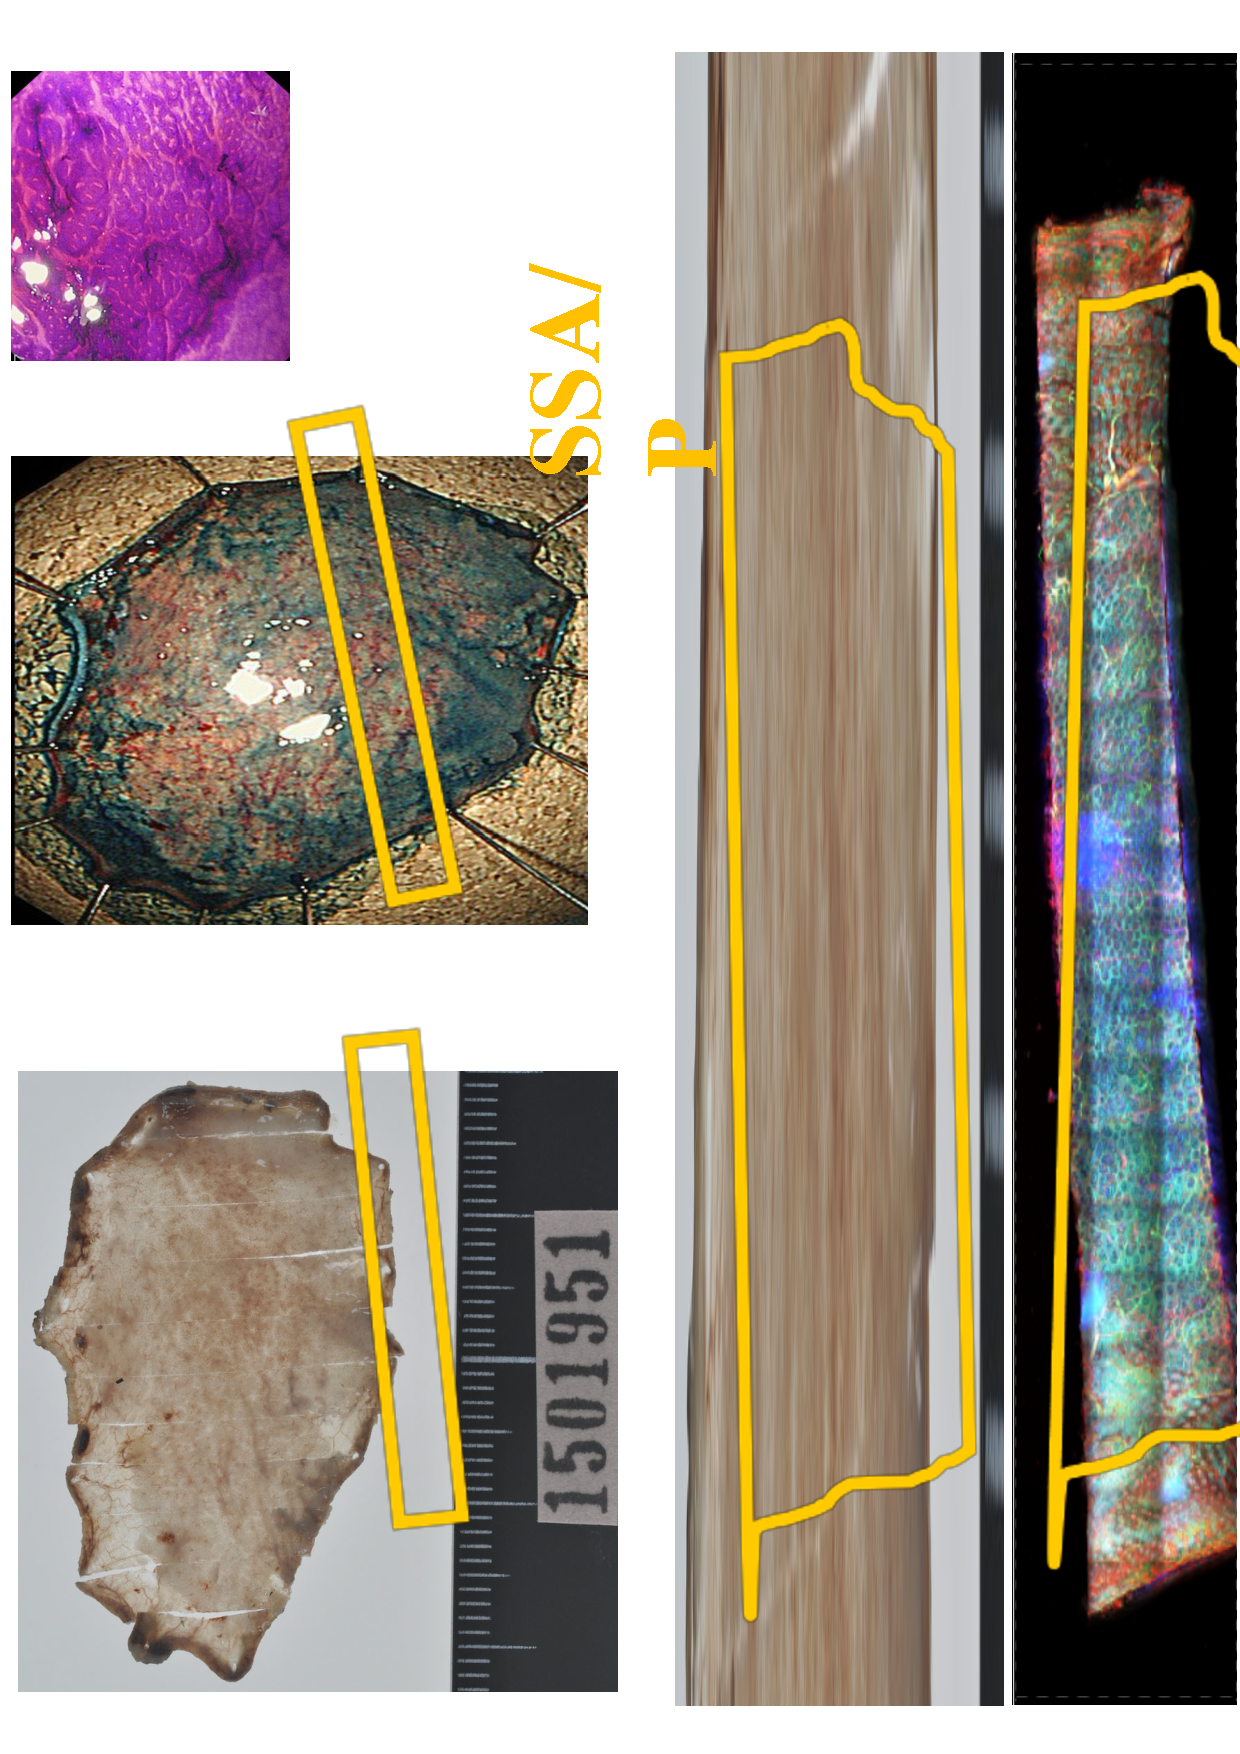
\includegraphics[clip, width=0.4\linewidth]{fig/raw_data/summary/C-010}
}
	\subfigure[]{
	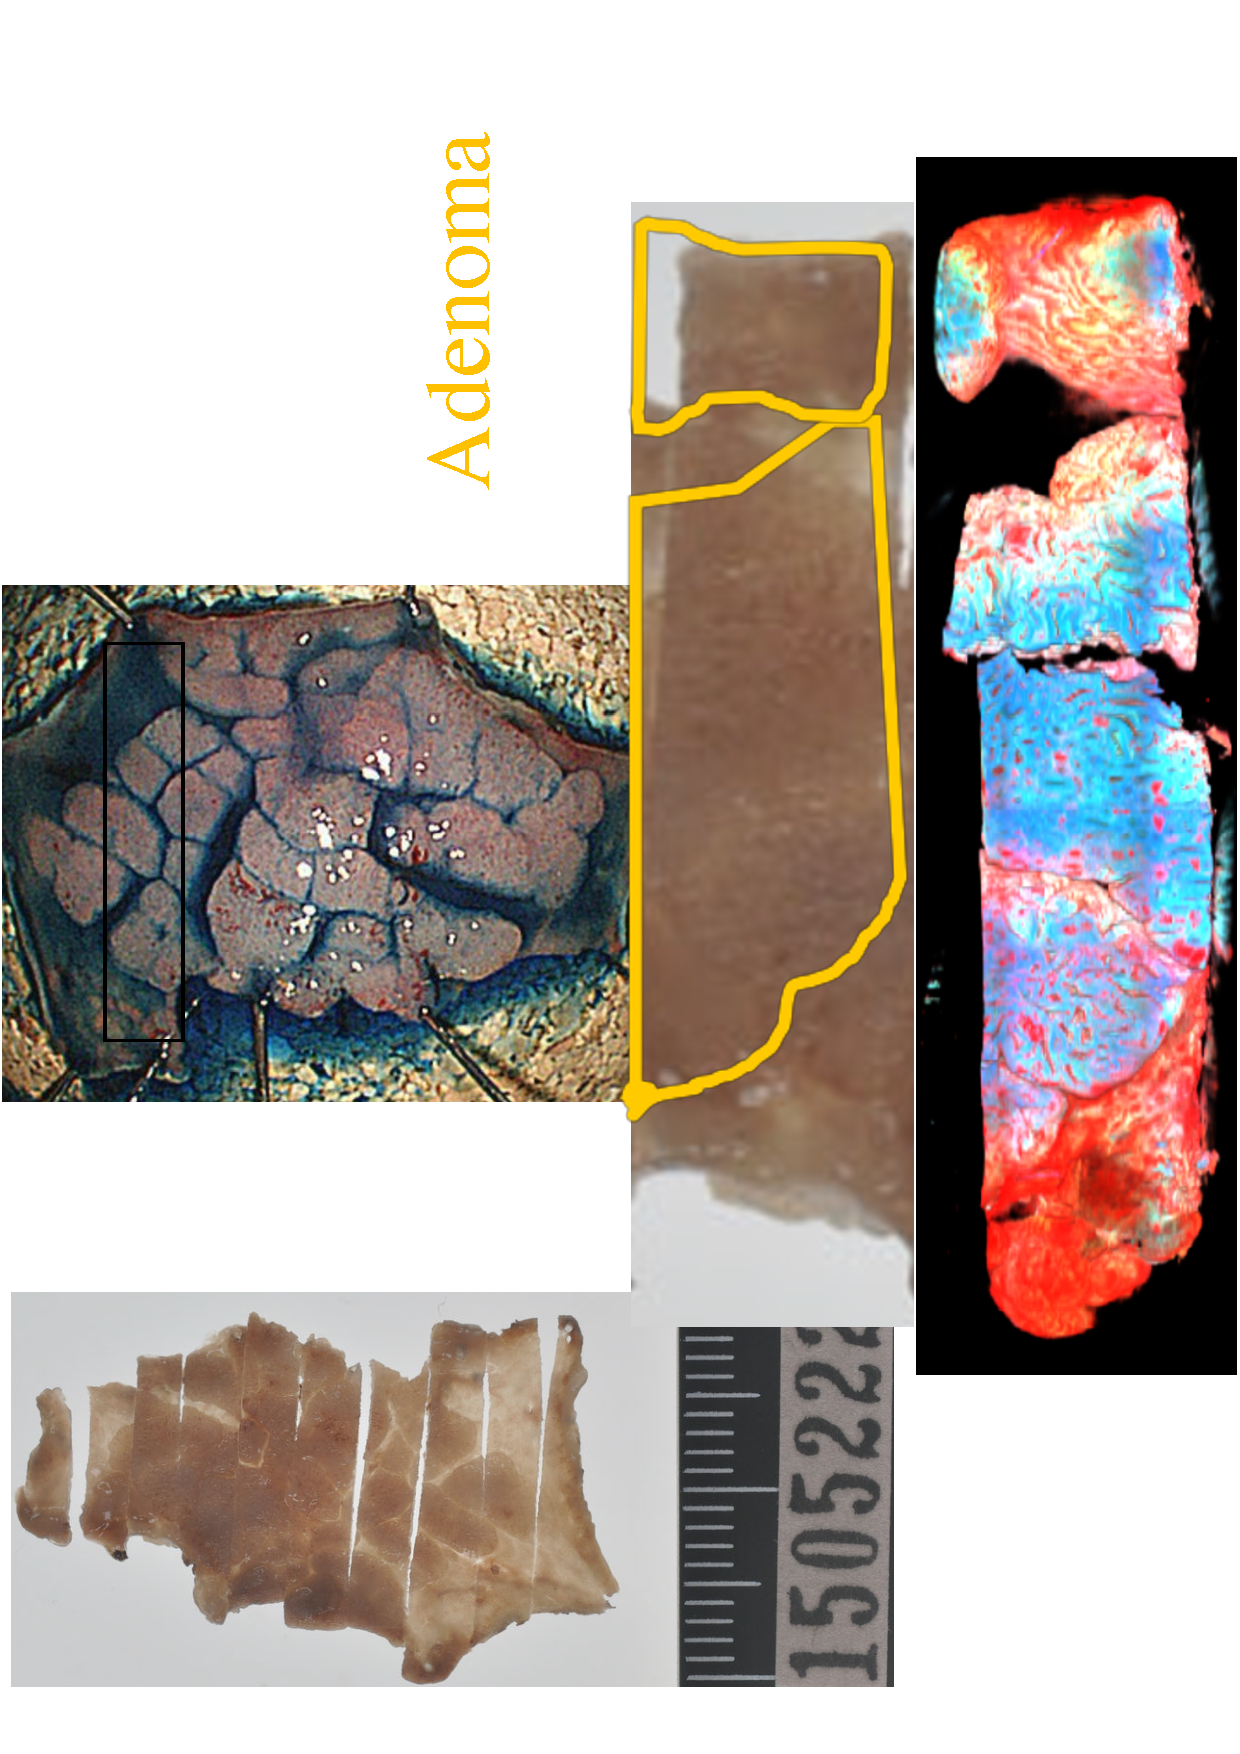
\includegraphics[clip, width=0.4\linewidth]{fig/raw_data/summary/C-011}
}
	\subfigure[]{
	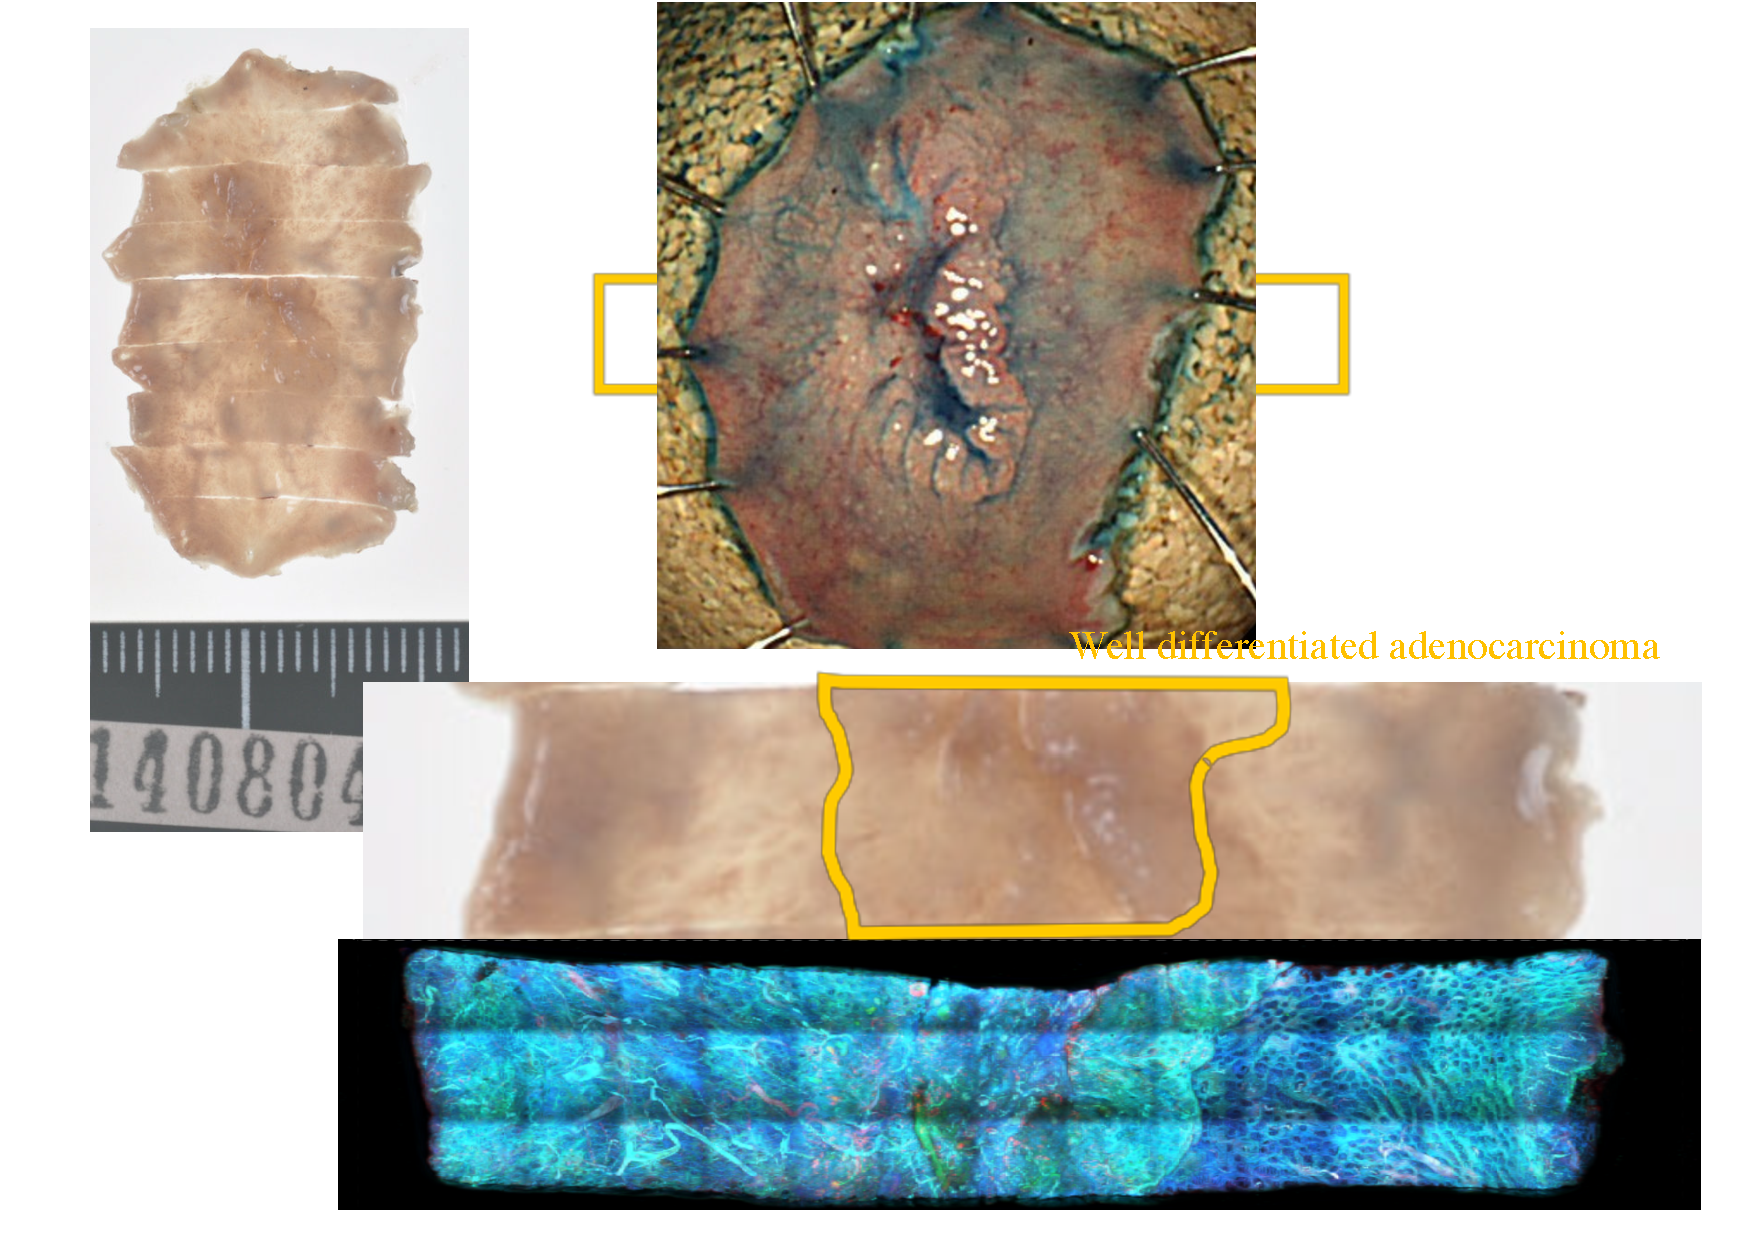
\includegraphics[clip, width=0.4\linewidth]{fig/raw_data/summary/C-013}
}
\end{figure}


\subsection{教師データの作成}
消化器内科の医師がつけた腫瘍部分を教師データとして利用した.以下の図が腫瘍の位置をマスクした画像になっている.

\begin{figure}
	\centering
	\subfigure[]{
	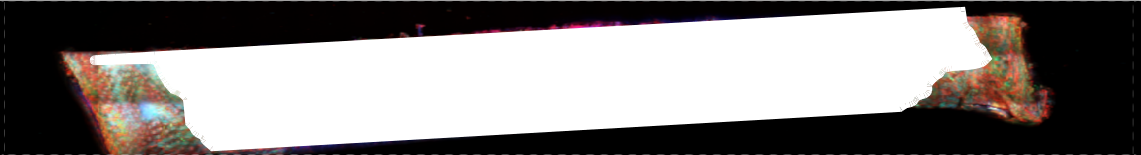
\includegraphics[clip, width=0.4\linewidth]{fig/raw_data/label/C-010}
	}
	\subfigure[]{
	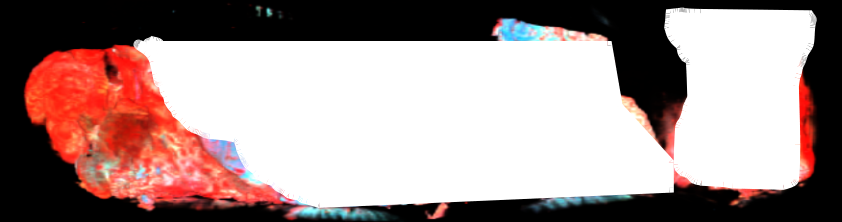
\includegraphics[clip, width=0.4\linewidth]{fig/raw_data/label/C-011}
}
	\subfigure[]{
	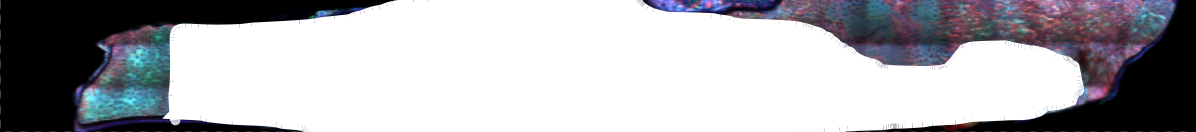
\includegraphics[clip, width=0.4\linewidth]{fig/raw_data/label/C-012}
}
	\subfigure[]{
	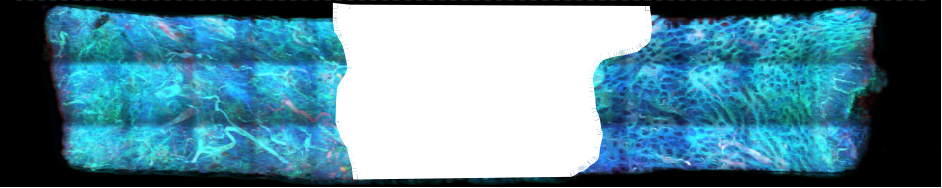
\includegraphics[clip, width=0.4\linewidth]{fig/raw_data/label/C-013}
}
\end{figure}

\section{前処理}

\subsection{擬似HE染色}
\begin{figure}
	\centering
	\subfigure[]{
		\includegraphics[clip, width=0.4\linewidth]{fig/preprocessing/pseudo-HE/0130171}
	}
	\subfigure[]{
	\includegraphics[clip, width=0.4\linewidth]{fig/preprocessing/pseudo-HE/0120100}
}
	\subfigure[]{
	\includegraphics[clip, width=0.4\linewidth]{fig/preprocessing/pseudo-HE/0100}
}
	\subfigure[]{
	\includegraphics[clip, width=0.4\linewidth]{fig/preprocessing/pseudo-HE/0110240}
}
\end{figure}

教師ラベルから,正常と腫瘍に分割した.
\begin{figure}
	\centering
	\subfigure[]{
		\includegraphics[clip, width=0.4\linewidth]{fig/preprocessing/separated_label/normal/normal_C-013}
	}
	\subfigure[]{
		\includegraphics[clip, width=0.4\linewidth]{fig/preprocessing/separated_label/cancer/cancer_C-013}
	}
\end{figure}

\section{Data Augmentation}
少量データセットであるため,少しの画像から,より多くの特徴を抽出するために,擬似的にデータの水増し(Data Augmentation)を行う.
注意した点は,入力画像としてあり得る範囲のバリエーションの中でデータ拡張を行った・

\subsection*{回転}
\begin{figure}
	\centering
	\subfigure[0°]{
		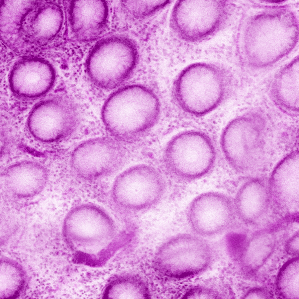
\includegraphics[clip, width=0.4\linewidth]{fig/preprocessing/data_aug/rotate/ROTATION_0}
	}
	\subfigure[90°]{
	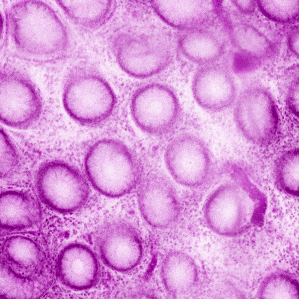
\includegraphics[clip, width=0.4\linewidth]{fig/preprocessing/data_aug/rotate/ROTATION_90}
}
	\subfigure[180°]{
	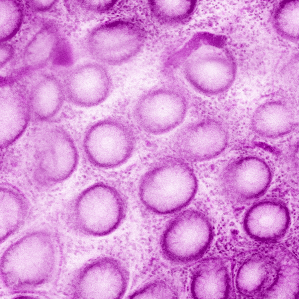
\includegraphics[clip, width=0.4\linewidth]{fig/preprocessing/data_aug/rotate/ROTATION_180}
}
	\subfigure[270°]{
	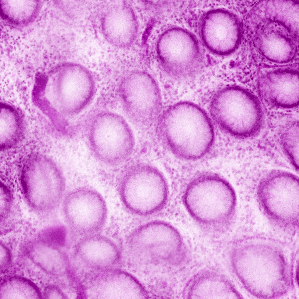
\includegraphics[clip, width=0.4\linewidth]{fig/preprocessing/data_aug/rotate/ROTATION_270}
}
\end{figure}

\subsection*{反転}
\begin{figure}
	\centering
	\subfigure[水平反転]{
		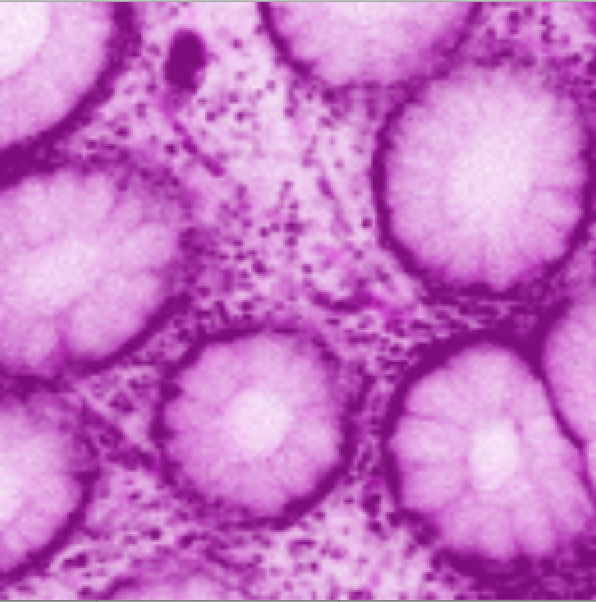
\includegraphics[clip, width=0.4\linewidth]{fig/preprocessing/data_aug/horizontal_flip/horizontal_flip}
	}
	\subfigure[垂直反転]{
		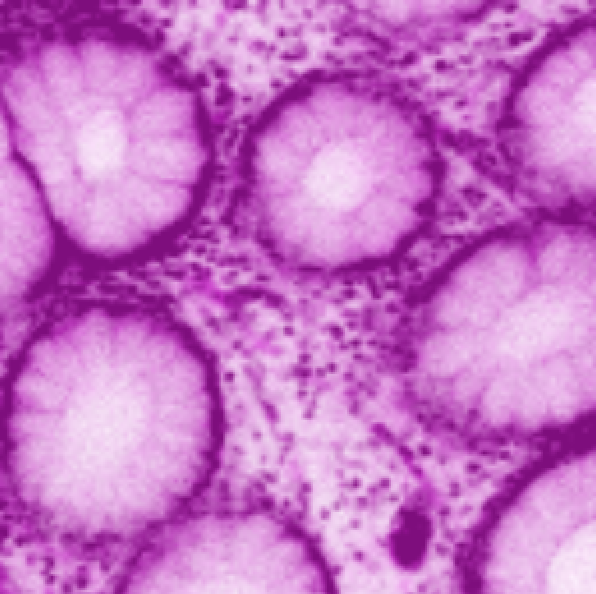
\includegraphics[clip, width=0.4\linewidth]{fig/preprocessing/data_aug/vertical_flip/vertical_flip}
	}
\end{figure}

\subsection*{ガウシアンブラー}
\begin{figure}
	\centering
	\subfigure[0]{
		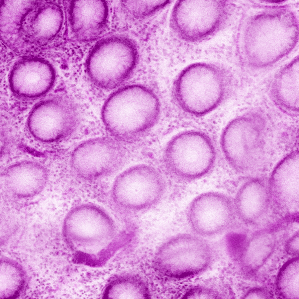
\includegraphics[clip, width=0.4\linewidth]{fig/preprocessing/data_aug/color/blur/blur_0_00}
	}
	\subfigure[0.5]{
		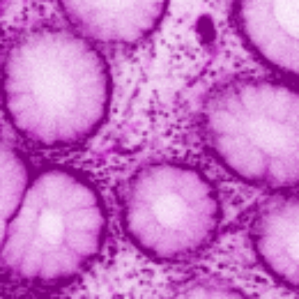
\includegraphics[clip, width=0.4\linewidth]{fig/preprocessing/data_aug/color/blur/blur_0_50}
	}
	\subfigure[1]{
		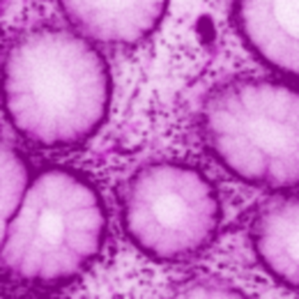
\includegraphics[clip, width=0.4\linewidth]{fig/preprocessing/data_aug/color/blur/blur_1_00}
	}
	\subfigure[2]{
		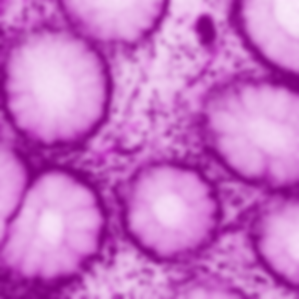
\includegraphics[clip, width=0.4\linewidth]{fig/preprocessing/data_aug/color/blur/blur_2_00}
	}
\end{figure}

\subsection*{鮮鋭度}
\begin{figure}
	\centering
	\subfigure[0]{
		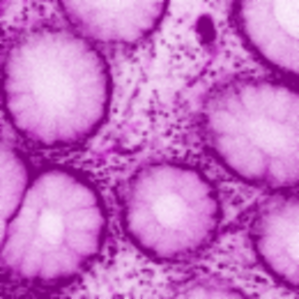
\includegraphics[clip, width=0.4\linewidth]{fig/preprocessing/data_aug/color/SHARPNESS/SHARPNESS_0_00}
	}
	\subfigure[0.5]{
		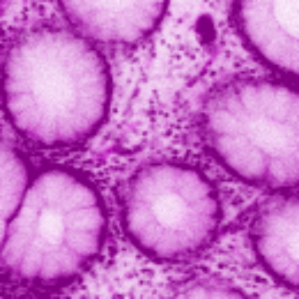
\includegraphics[clip, width=0.4\linewidth]{fig/preprocessing/data_aug/color/SHARPNESS/SHARPNESS_0_50}
	}
	\subfigure[1]{
		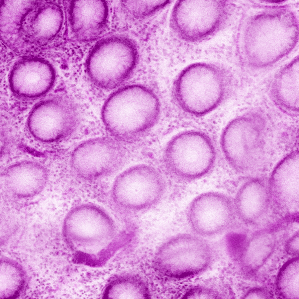
\includegraphics[clip, width=0.4\linewidth]{fig/preprocessing/data_aug/color/SHARPNESS/SHARPNESS_1_00}
	}
	\subfigure[2]{
		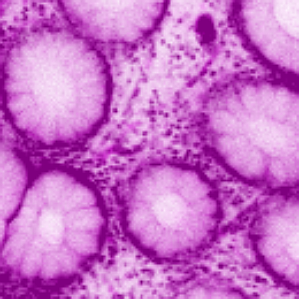
\includegraphics[clip, width=0.4\linewidth]{fig/preprocessing/data_aug/color/SHARPNESS/SHARPNESS_2_00}
	}
\end{figure}

\subsection*{輝度}
\begin{figure}
	\centering
	\subfigure[0.8]{
		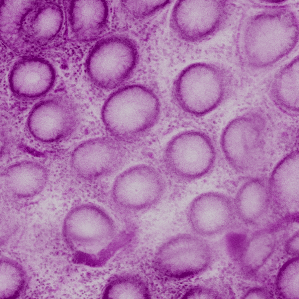
\includegraphics[clip, width=0.4\linewidth]{fig/preprocessing/data_aug/color/BRIGHTNESS/BRIGHTNESS_0_80}
	}
	\subfigure[1.0]{
		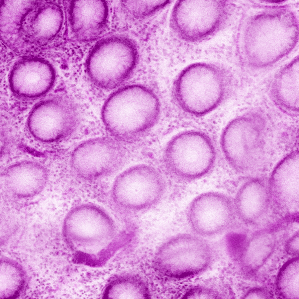
\includegraphics[clip, width=0.4\linewidth]{fig/preprocessing/data_aug/color/BRIGHTNESS/BRIGHTNESS_1_00}
	}
	\subfigure[1.2]{
		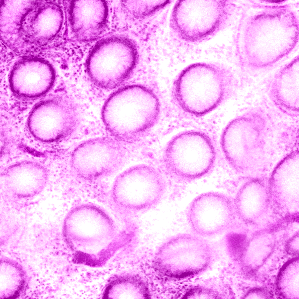
\includegraphics[clip, width=0.4\linewidth]{fig/preprocessing/data_aug/color/BRIGHTNESS/BRIGHTNESS_1_20}
	}
\end{figure}

\subsection*{コントラスト}
\begin{figure}
	\centering
	\subfigure[0.5]{
		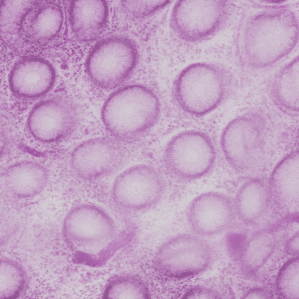
\includegraphics[clip, width=0.4\linewidth]{fig/preprocessing/data_aug/color/CONTRAST/CONTRAST_0_50}
	}
	\subfigure[1.0]{
		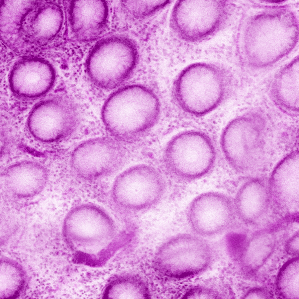
\includegraphics[clip, width=0.4\linewidth]{fig/preprocessing/data_aug/color/CONTRAST/CONTRAST_1_00}
	}
	\subfigure[1.5]{
		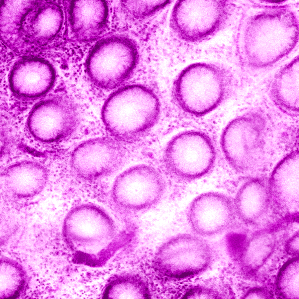
\includegraphics[clip, width=0.4\linewidth]{fig/preprocessing/data_aug/color/CONTRAST/CONTRAST_1_50}
	}
\end{figure}

\subsection*{彩度}
\begin{figure}
	\centering
	\subfigure[0.5]{
		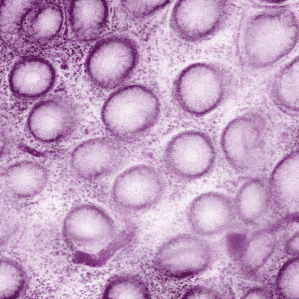
\includegraphics[clip, width=0.4\linewidth]{fig/preprocessing/data_aug/color/SATURATION/SATURATION_0_50}
	}
	\subfigure[1.0]{
		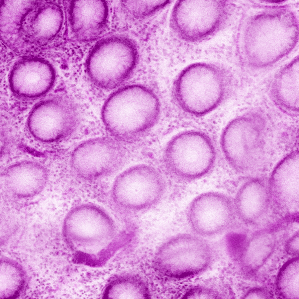
\includegraphics[clip, width=0.4\linewidth]{fig/preprocessing/data_aug/color/SATURATION/SATURATION_1_00}
	}
	\subfigure[1.5]{
		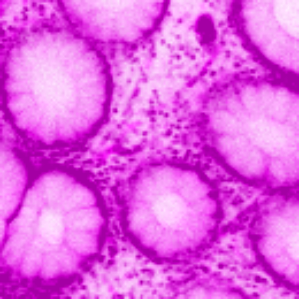
\includegraphics[clip, width=0.4\linewidth]{fig/preprocessing/data_aug/color/SATURATION/SATURATION_1_50}
	}
\end{figure}

\section{古典的な画像処理手法による識別精度評価}
正常と腫瘍を両方含む画像に対してHough変換による円検出で正常の線管構造を検出した.円検出では検出できない線菅構造をより多く検出するために楕円でも検出ができるように変更した.複数のパラメータを調整することで,アノテーションの正常領域が検出できるような円検出の数を増やしながらも,ノイズが多くならないような値を決定した.また,これが複数の検体で試してみた時に,最適なパラメータを見積もった.

\section{事前学習}
今回のように新しい画像の撮影方法でデータを多く集めることができない時は,類似データを事前に学習しておく事前学習を用いる.
大腸の管構造の特徴を捉えるために,外部のデータセットのGland Challengeデータセットを使って事前学習を行う.

\section{教師あり学習による識別精度評価}
\subsection*{2次元画像}
\subsection*{3次元画像}

\section{教師なし学習による識別精度評価}
\subsection*{2次元画像}
\subsection*{3次元画像}

\section{半教師あり学習による識別精度評価}
\subsection*{2次元画像}
\subsection*{3次元画像}

\section{学習環境}
Ubuntu 14.04
Github
